\subsubsection{Mostrant els detalls d'una persona}

\paragraph{}
La selecció d'una persona, a la taula de resultats originada per la cerca, provoca una segona crida al SDK de FamilySearch en la que s'obté tota la informació disponible sobre la persona seleccionada i els seus familiars.

Com en totes les crides a l'API, en cas d'error, aquest és mostrat en una secció específica. En cas d'èxit, es pinta, en diferents taules, la informació bàsica de la persona, els diferents noms pels quals és coneguda, els esdeveniments relacionats amb la seva vida, informació bàsica sobre els seus pares, parelles i fills, informació de la seva ascendència i descendència, notes de FamilySearch, fonts de dades que verifiquen la informació mostrada i l'historial de canvis realitzat sobre la persona.

Es mostra en la figura~\ref{fig:personSearchDetails}, l'inici de la secció de taules resultant de demanar els detalls específics d'una persona.

\begin{figure}[h]
    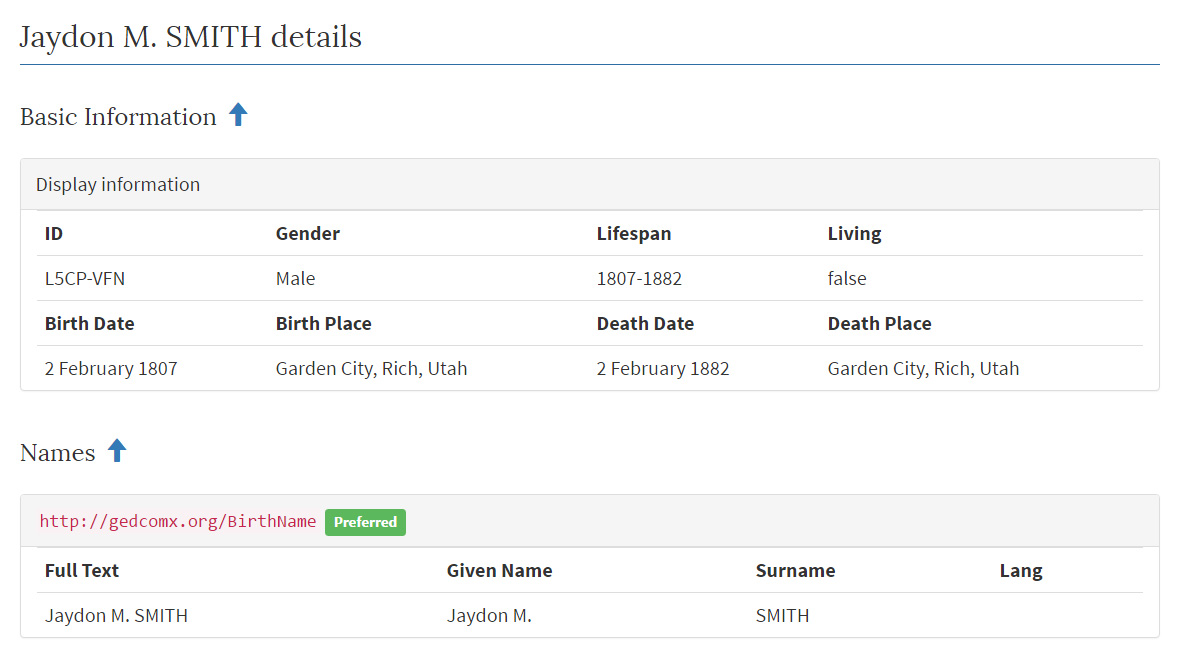
\includegraphics[width=\linewidth]{11/02_searchPersons/02_personDetails}
    \centering
    \caption{Exemples de l'inici dels detalls d'una persona}\label{fig:personSearchDetails}
\end{figure}

La crida a l'API que gestiona aquesta informació és mostra en el següent bloc de codi.

\begin{lstlisting}[style=rawOwn,caption={Crida al SDK per obtenir tota la informació d'una persona}]
client.getPersonWithRelationships(personID).then(function(personResponse) {
    var mainPerson = personResponse.getPrimaryPerson();
    personDisplayProperties(mainPerson);
    personDisplayNames(mainPerson.getNames());
    personDisplayFacts(mainPerson.getFacts());
    ...
    client.getAncestry( ... );
    client.getDescendancy( ... );
    ...
    mainPerson.getChanges( ... );
});
\end{lstlisting}

Com s'ha pogut observar en el bloc de codi anterior, per obtenir les diferents peces d'informació, s'ha de navegar per diferents nivells de la resposta. Alguna informació és accessible directament des de l'objecte inicial, mentre que alguns altres paràmetres cal anar a buscar-los a l'objecte específic de la persona. Per altra banda, la informació relativa a l'ascendència i descendència, cal demanar-la de forma explícita al SDK.

Les dades retornades per les crides al SDK, sobre l'ascendència i descendència, esdevenen interessants, ja que la navegació pels resultats es realitza mitjançant la nomenclatura `Ahnentafel' i `Aboville' respectivament.

La nomenclatura `Anhentafel', atorga a la persona sobre la qual se cerca l'ascendència, el nombre 1. El seu pare, rep el número 2 i la mare, el 3. Les regles per calcular els nombres dels pares de qualsevol persona en l'ascendència són:

\begin{itemize}
    \item \textbf{Pare:} nombre de la persona $\times$ 2
    \item \textbf{Mare:} nombre de la persona $\times$ 2 + 1
\end{itemize}

Per altra banda, la nomenclatura `Aboville', utilitza una estructura similar a la de les seccions i apartats d'aquesta memòria. Si s'atorga el nombre 1, a la persona sobre la qual se cerca la descendència, s'utilitza per les diferents generacions:

\begin{itemize}
    \item \textbf{Fills:} 1.1 / 1.2 / 1.3 / etcètera.
    \item \textbf{Els fills dels fill 1.1:} 1.1.1 / 1.1.2 / 1.1.3 / etcètera.
    \item \textbf{Els fills del fill 1.2 del fill 1.1:} 1.1.2.1 / 1.1.2.2 / etcètera.
\end{itemize}
